\chapter{Diseño e implementación} % Main chapter title

\label{Chapter3} % Change X to a consecutive number; for referencing this chapter elsewhere, use \ref{ChapterX}

En este capítulo, se presentan de manera concisa las decisiones de diseño del sistema. 
Se abordan aspectos clave como la adquisición de datos, las técnicas de preprocesamiento 
utilizadas y el diseño del modelo de aprendizaje profundo. 

%----------------------------------------------------------------------------------------
%	ADQUISICION DE DATOS
%----------------------------------------------------------------------------------------
\section{Adquisición de datos}
 
\newcommand{\myhash}{\raisebox{\depth}{\#}}

Para llevar a cabo el presente trabajo, se emplearon datos proporcionados por el servicio 
de cardiología e hipertensión del Hospital Alemán. La figura \ref{fig:adquisicion_datos} 
exhibe un diagrama en bloques que ilustra la etapa de adquisición de datos utilizada. 
Es importante destacar que se utilizaron dos conjuntos de datos diferentes. 

\begin{figure}[ht]
	\centering
	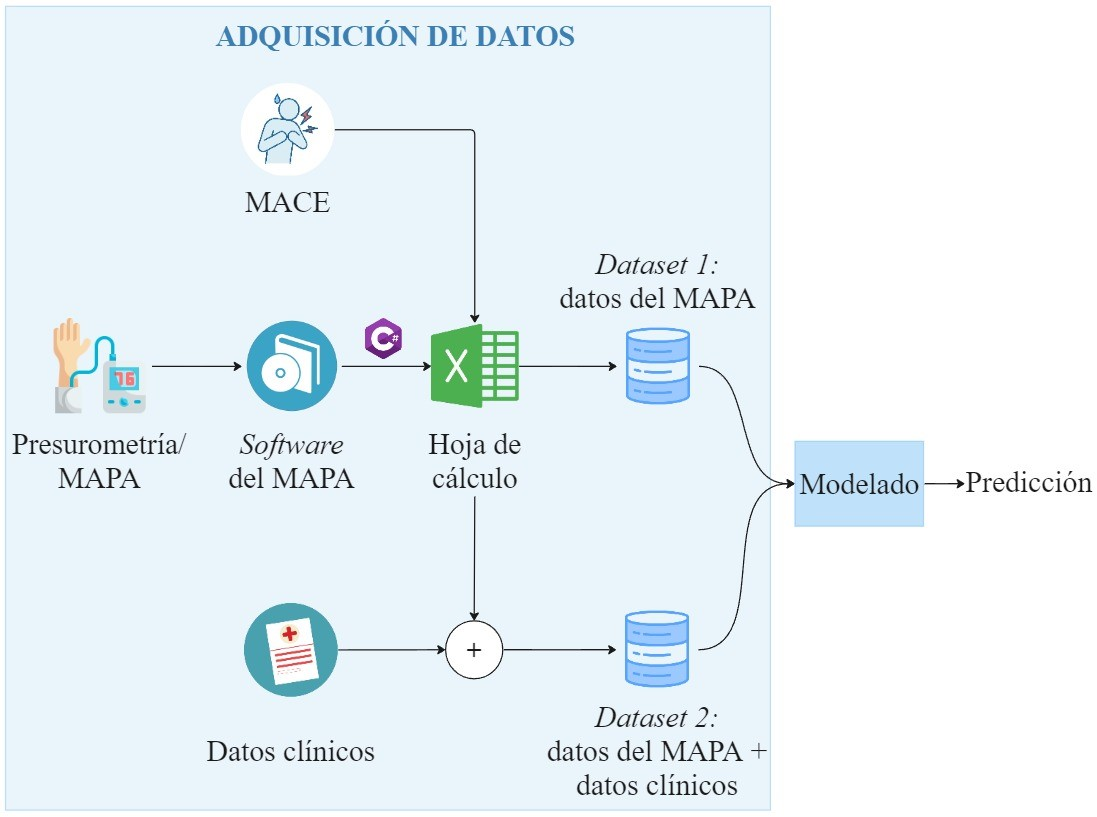
\includegraphics[width=\textwidth]{./Figures/adquisicion_datos2.jpg}
	\caption{Representación esquemática de la etapa de adquisición de datos.}\label{fig:adquisicion_datos}
\end{figure}

El primer \emph{dataset} se compone exclusivamente de información recopilada de las 
presurometrías realizadas a los pacientes hipertensos a partir del año 2013. Luego 
de realizar un MAPA, los datos se almacenan en un \emph{software} especializado de 
los presurómetros. Posteriormente, se extraen utilizando un programa desarrollado 
en C\# para ser registrados en una planilla de cálculo. Sumado a esto, se incluyó 
la variable a predecir (MACE) para cada paciente mediante un análisis exhaustivo 
de su historial clínico. Especificamente, se registró la ocurrencia de 
un accidente cerebrovascular no fatal, infarto agudo de miocardio, insuficiencia 
cardíaca, insuficiencia renal crónica o muerte. En caso de que correspondiera, también 
se incluyó la fecha correspondiente en la que tuvo lugar el evento.

Por otro lado, el segundo conjunto de datos contiene información adicional obtenida 
del historial clínico de cada paciente. Estos datos clínicos se agregan a la misma 
hoja de cálculo mencionada anteriormente, complementando así la información proveniente 
de las presurometrías.

El objetivo de utilizar dos \emph{datasets} es evaluar la calidad de los datos de 
las presurometrías para generar inferencias de manera independiente. En otras palabras, 
se buscó determinar en qué medida los datos del MAPA pueden ser utilizados por sí solos 
para obtener predicciones significativas y precisas de MACE. Al mismo tiempo, se procuró 
evaluar si la incorporación de información clínica contribuye a un mejor desempeño del 
modelo en términos de tasa de falsos negativos, AUC y otras métricas relevantes.


%----------------------------------------------------------------------------------------
% 3.1.1 Descripción del conjunto de datos

\subsection{Descripción del conjunto de datos}

El primer conjunto de datos comprende las variables derivadas del MAPA, junto con 
el valor de MACE y la fecha del evento asociado. A continuación, se brinda una 
descripción detallada de las variables provenientes de las presurometrías: 

\begin{itemize}
  \item Fechaest: corresponde a la fecha en la cual se realizó la presurometría.
  \item PASm24: representa la presión arterial sistólica media durante todo el MAPA.
	\item PADm24: representa la presión arterial diastólica media durante todo el MAPA.
  \item FCm24: representa la frecuencia cardíaca media durante todo el MAPA.
  \item PAMm24: representa la presión arterial media durante todo el MAPA.
  \item PPm24: representa la presión de pulso media durante todo el MAPA.
  \item PASsd24: indica el desvío estándar de la presión arterial sistólica media durante todo el MAPA. 
  \item PADsd24: indica el desvío estándar de la presión arterial diastólica media durante todo el MAPA.
  \item FCsd24:  indica el desvío estándar de la frecuencia cardíaca media durante todo el MAPA.
  \item PAMsd24: indica el desvío estándar de la presión arterial media durante todo el MAPA.
  \item PPsd24: indica el desvío estándar de la presión de pulso media durante todo el MAPA.
  \item PASmDIA: representa la presión arterial sistólica media diurna.
  \item PADmDIA: representa la presión arterial diastólica media diurna.
  \item FCmDIA: representa la frecuencia cardíaca media diurna.
  \item PAMmDIA: representa la presión arterial media diurna.
  \item PPmDIA: representa la presión de pulso media diurna.
  \item htaloadsbpDIA: se refiere al porcentaje de lecturas de la presión arterial sistólica que exceden el valor de referencia de 135 mmHg durante el día.
  \item htaloaddbpDIA: se refiere al porcentaje de lecturas de la presión arterial diastólica que exceden el valor de referencia de 85 mmHg durante el día.
  \item HTAdia01: se utiliza para determinar si un paciente presenta hipertensión diurna (HTAdia01 = 1) o normotensión diurna (HTAdia01 = 0). Se considera hipertensión diurna cuando la presión arterial sistólica es superior a 135 mmHg y la presión arterial diastólica es superior a 85 mmHg durante el día, mientras que se define como normotensión diurna cuando no se cumplen estos criterios.
  \item PASmNOCHE: representa la presión arterial sistólica media nocturna.
  \item PADmNOCHE: representa la presión arterial diastólica media nocturna.
  \item FCmNOCHE: representa la frecuencia cardíaca media nocturna.
	\item PAMmNOCHE: representa la presión arterial media nocturna.
	\item PPmNOCHE: representa la presión de pulso media nocturna.
  \item htaloadsbpNOCHE: representa el porcentaje de lecturas de la presión arterial sistólica que exceden el valor de referencia de 125 mmHg durante la noche.
  \item htaloaddbpNOCHE: se refiere al porcentaje de lecturas de la presión arterial diastólica que exceden el valor de referencia de 70 mmHg durante la noche.
  \item HTAnoche01: se define como hipertensión nocturna (HTAnoche01 = 1) cuando la presión arterial sistólica es superior a 120 mmHg y la presión arterial diastólica es superior a 70 mmHg durante la noche. En caso contrario, se considera normotensión nocturna (HTAnoche01 = 0).
  \item Nondipper01: se utiliza para clasificar a los pacientes en función de la disminución de la presión arterial nocturna. Cuando la presión arterial no disminuye en un 10\% durante la noche, se considera un indicador de alto riesgo cardiovascular y se denominan \emph{non-dippers} (Nondipper01 = 1). Por otro lado, aquellos pacientes cuya presión arterial disminuye en un 10\% durante la noche se denominan \emph{dippers} (Nondipper01 = 0).
\end{itemize}


El segundo conjunto de datos, por su parte, incluye todas las variables mencionadas anteriormente, junto con
9 variables adicionales extraídas del historial clínico de cada paciente. Estas incluyen:

\begin{itemize}
  \item Talla: se refiere a la medida de la longitud del cuerpo de una persona y se expresa en centímetros.
  \item Peso: se refiere a la medida de la masa corporal del paciente expresada en kilogramos.
  \item IMC: el índice de masa corporal (IMC) es una medida utilizada para evaluar la relación entre el peso y la estatura de una persona. Se calcula dividiendo el peso en kilogramos por el cuadrado de la estatura en metros.
  \item Edad: representa el tiempo transcurrido desde el nacimiento de un individuo, medido en años.
  \item Sexo: indica si el paciente es hombre (Sexo = 0) o mujer (Sexo = 1).
  \item DBT: indica la presencia (DBT = 1) o ausencia (DBT = 0) de diabetes en un paciente, una enfermedad metabólica crónica caracterizada por niveles elevados de glucosa en sangre.
  \item Tabaquismo: indica si un paciente tiene adicción a la nicotina (Tabaquismo = 1) o no presenta dicha adicción (Tabaquismo = 0).
  \item Dislipemia: señala la presencia (Dislipemia = 1) o ausencia (Dislipemia = 0) de una alteración en los niveles de lípidos en sangre en un paciente.
  \item HVI: indica la presencia (HVI = 1) o ausencia (HVI = 0) de un engrosamiento de la pared del ventrículo izquierdo como consecuencia de la hipertensión en el paciente.
\end{itemize}

%------------------------------------------------------------------------
%	PREPROCESAMIENTO DE DATOS
%----------------------------------------------------------------------------------------
\section{Preprocesamiento de datos}
En la siguiente sección, se proporciona una descripción detallada del preprocesamiento de datos 
realizado en este trabajo. El objetivo principal de esta etapa fue la obtención de un conjunto de 
datos final de alta calidad y utilidad para su posterior análisis y modelado. En la subsección 
\ref{sec:Conjunto1} se describe el procesamiento realizado al conjunto de datos de presurometrías. 
Posteriormente, en la subsección \ref{sec:Conjunto2} se aborda el procesamiento 
llevado a cabo en el conjunto de datos que combina los datos de MAPA y los datos clínicos.

%------------------------------------------------------------------------
%	datos presurometrias
%%%%%%%%%%%%%%%%%%%%%%%
\subsection{Conjunto de datos de presurometrías}
\label{sec:Conjunto1}

El conjunto de datos utilizado consta de 491 informes de MAPA y se caracteriza por no tener datos faltantes. 
Este \emph{dataset} incluye: 3 variables categóricas (HTA durante el día, HTA durante la noche y \emph{non-dipper}), 
2 variables de fecha (fecha del estudio y fecha de MACE) y 25 variables numéricas continuas.


\subsubsection{Distribuciones de las variables numéricas}
Se realizó un análisis de las distribuciones de los datos con el objetivo de determinar si siguen una distribución 
normal y si existen valores extremos. 

En primer lugar, se llevaron a cabo pruebas visuales utilizando gráficos Q-Q 
(cuantil-cuantil) e histogramas. El gráfico Q-Q es una herramienta utilizada para comparar dos distribuciones de 
probabilidad trazando sus cuantiles uno contra el otro. Aunque no es una prueba estadística formal, proporciona 
una forma sencilla e intuitiva de verificar qué distribución sigue un conjunto de datos. Por otro lado, el 
histograma permite visualizar la distribución de frecuencias de los datos de una variable. En la figura \ref{fig:qqplots} 
se presentan los gráficos Q-Q y los histogramas de las presiones y la frecuencia cardíaca media durante 24 horas, 
así como de las cargas hipertensivas sistólicas y diastólicas durante el día y la noche. Se observa que la PAD, 
PAM y frecuencia cardíaca (FC) siguen una distribución normal. Sin embargo, la PAS y PP muestran una 
ligera sesgadura hacia la derecha. Aunque no se exhiben en la figura \ref{fig:qqplots}, las presiones y FC 
mencionadas anteriormente presentan la misma distribución durante el día y la noche. 
Por otro lado, las cargas hipertensivas sistólicas presentan una distribución asimétrica a la derecha, 
mientras que las cargas hipertensivas diastólicas presentan una distribución casi uniforme.

\begin{figure}[ht]
	\centering
	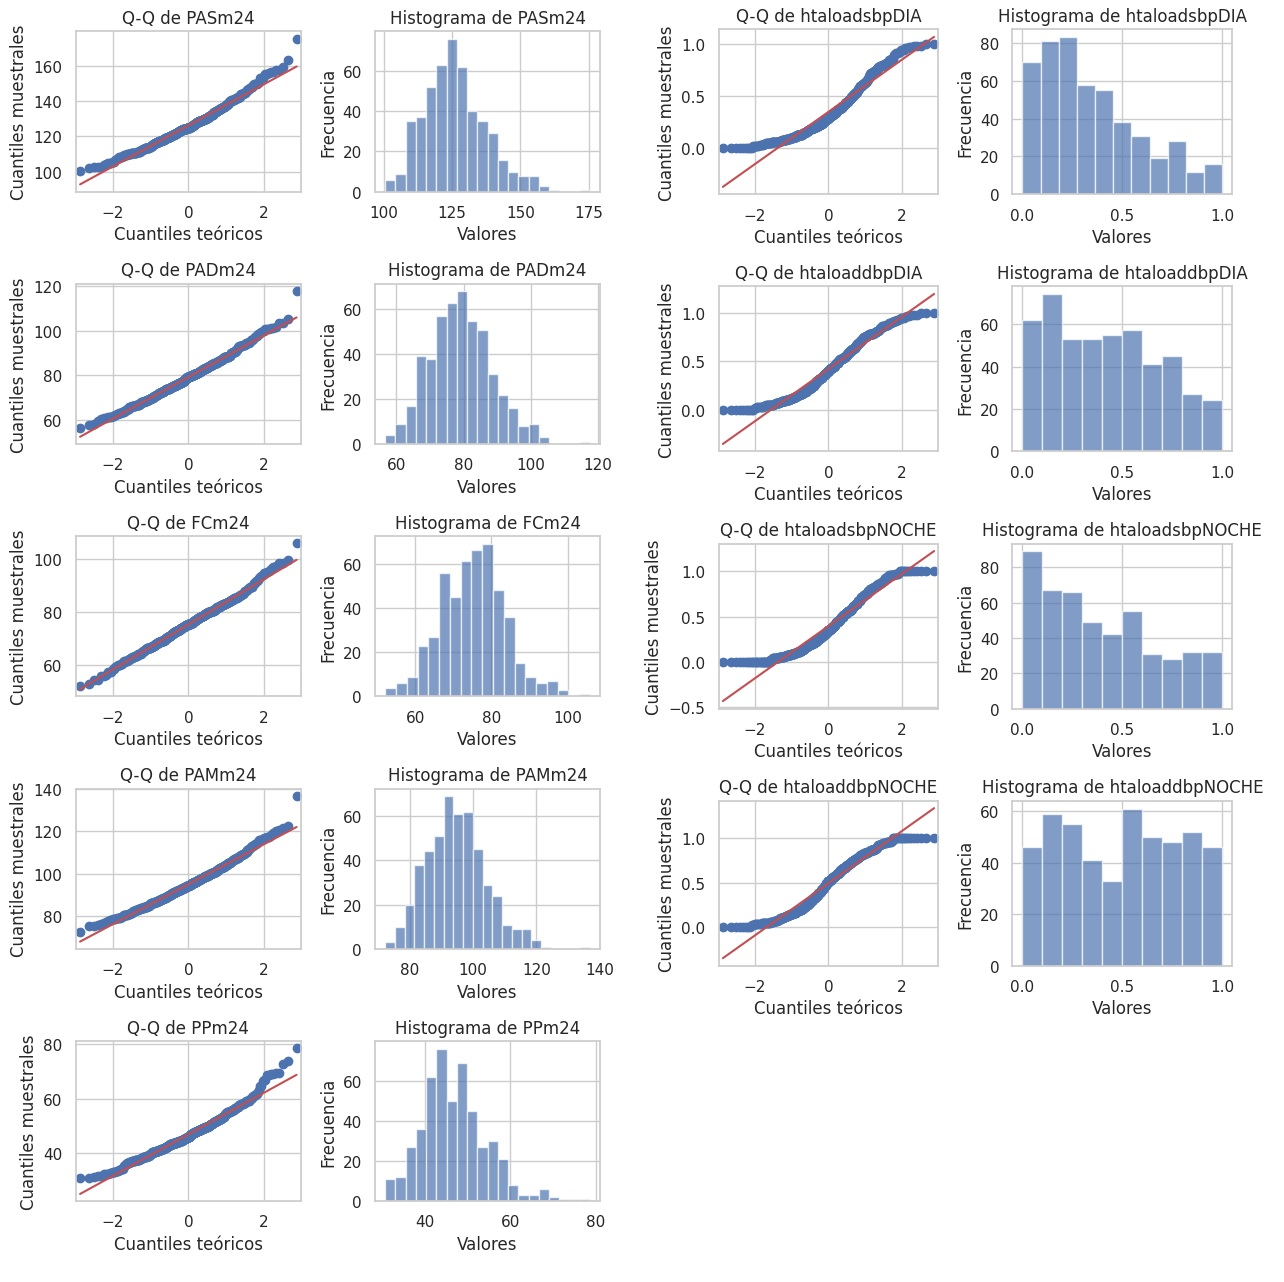
\includegraphics[width=\textwidth]{./Figures/qqplots.jpg}
	\caption{Gráficos Q-Q e histogramas de la PAS, PAD, FC, PAM y PP durante 24 h; y cargas hipertensivas sistólicas y diastólicas durante el día y la noche.}\label{fig:qqplots}
\end{figure}


%%%%%%%%%%%%%%%%%%%%%%%
%%%%%%%%%%%%%%%%%%%%%%%
\subsubsection{Tratamiento de clases desbalanceadas }
En el contexto de este trabajo, se identificó un desbalance de clases, lo cual significa que una de las clases 
está representada por una fracción muy pequeña de las muestras totales. En la figura \ref{fig:desbalance_a} se puede 
observar que solamente un 7.54\% de las muestras pertenecen a la clase positiva, lo que equivale a 37 pacientes con MACE = 1. 
Este desequilibrio en las clases es un fenómeno intrínseco y esperable, ya que refleja la naturaleza del proceso 
que genera los datos. Sin embargo, el desbalance de clases puede crear un sesgo en el modelo de aprendizaje 
automático, ya que tiende a favorecer la predicción de la clase mayoritaria en lugar de capturar adecuadamente 
las instancias de la clase minoritaria. 

Para mitigar este problema, existen diversas técnicas que permiten equilibrar las clases en el conjunto de datos. 
En particular, para este trabajo se empleó la técnica SMOTE, la cual consiste en generar de forma sintética nuevos 
ejemplos de la clase minoritaria. De esta forma, se logró abordar de manera más precisa y equitativa el desafío 
de la predicción en un escenario desbalanceado. El nuevo conjunto de datos balanceado se exhibe en la figura \ref{fig:desbalance_b}.


\begin{figure}[h!]
	\centering
	\hspace{1em}
	\subcaptionbox{Conjunto de datos desbalanceado.\label{fig:desbalance_a}}
	[0.45\linewidth]{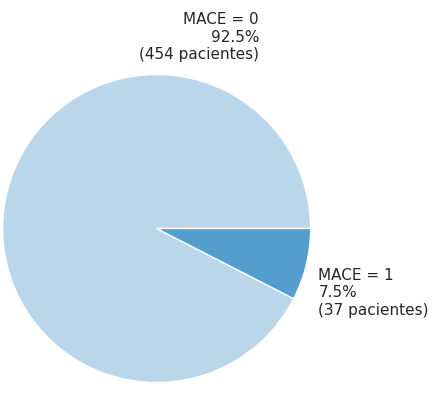
\includegraphics[height=6cm]{./Figures/desbalance_pie.png}}
	\hspace{1em}
	\subcaptionbox{Conjunto de datos después de emplear SMOTE.\label{fig:desbalance_b}}
	[0.45\linewidth]{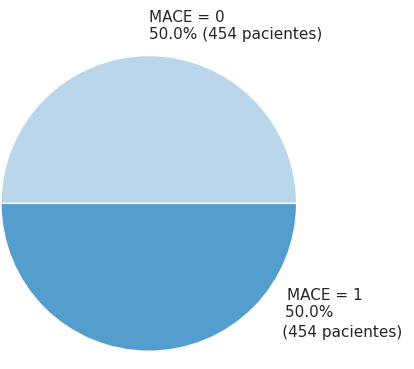
\includegraphics[height=5.5cm]{./Figures/desbalance_smote_pie.png}}
	\caption{Conjunto de datos antes y después de aplicar SMOTE.}
\end{figure}

%%%%%%%%%%%%%%%%%%%%%%%
%%%%%%%%%%%%%%%%%%%%%%%
\subsubsection{Normalización de características}
La normalización de los datos es un paso crucial antes de entrenar una red neuronal, y tiene como 
objetivo principal igualar la escala de las características de entrada. Esto es importante puesto 
que las redes neuronales son sensibles a las diferencias de escala entre las variables. En otras 
palabras, cuando los datos presentan diferentes escalas, algunas características con valores numéricos 
más altos pueden tener un impacto desproporcionado en el proceso de entrenamiento. De esta forma, 
esto puede ocasionar una mayor influencia en los pesos de la red y distorsionar el modelo resultante. 
Además, las funciones de activación utilizadas en las neuronas pueden funcionar de manera óptima 
cuando los datos están normalizados en un rango adecuado.

En este trabajo, se decidió utilizar el método \emph{StandardScaler} de \emph{scikit-learn} \citep{CITE:50} para 
normalizar las características de entrada. Este método aplica una transformación que ajusta la 
media de cada característica a 0 y la desviación estándar a 1. La definición de la transformación 
se muestra en la ecuación \ref{eq:normalizacion}, donde $X$ representa la matriz de características de 
entrada, $\mu$ a la media y $\sigma$ al desvío estándar. 

\begin{equation}
	\label{eq:normalizacion}
	X_{\text{normalizado}} = \frac{X - \mu}{\sigma}
\end{equation}

Al normalizar los datos de esta manera, se garantiza que todas las características tengan la 
misma escala, lo que facilita el proceso de aprendizaje de la red neuronal y mejora la convergencia 
del modelo. En la figura \ref{fig:normalizacion} se muestran a modo de ejemplo las distribuciones de 
la PAS, PAD y FC medias durante 24 horas antes y después de ser normalizadas. 

\begin{figure}[h!]
	\centering
	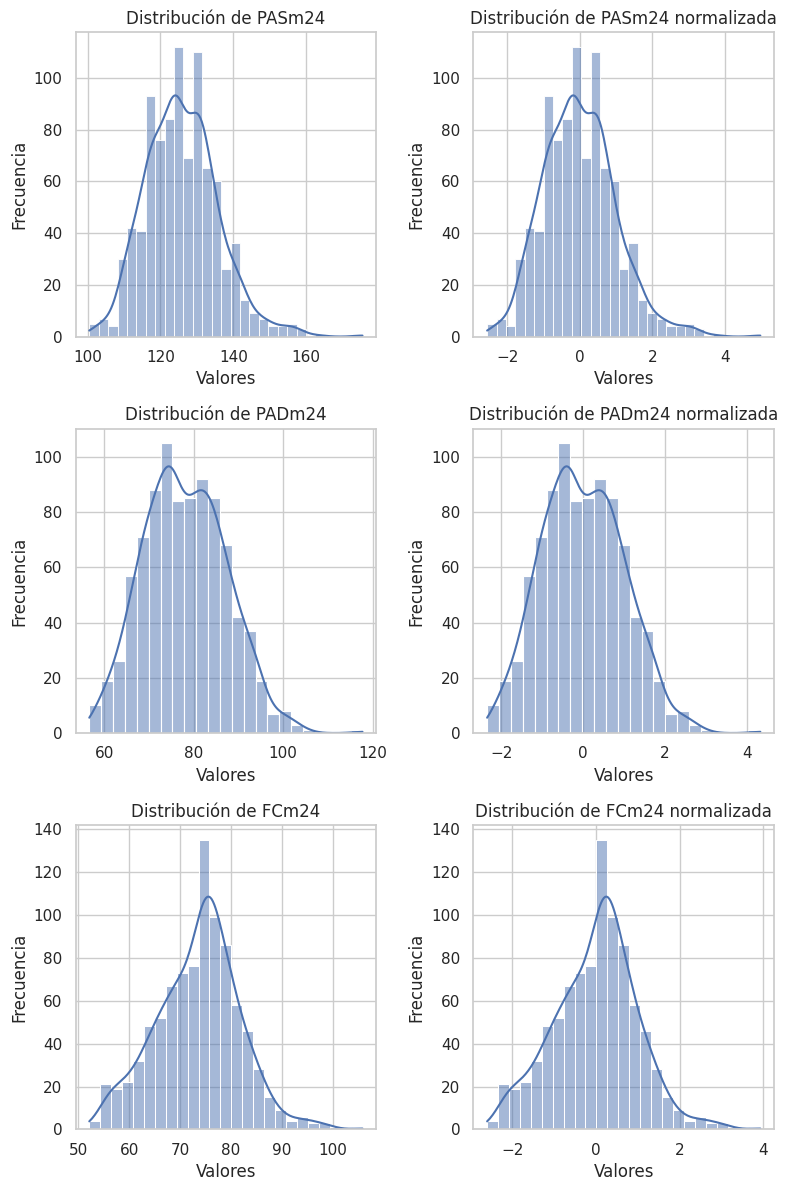
\includegraphics[width=0.8\textwidth]{./Figures/normalizacion.png}
	\caption{Distribuciones de la PAS, PAD y FC durante 24 h \\antes y después de la normalización.}\label{fig:normalizacion}
\end{figure}

%%%%%%%%%%%%%%%%%%%%%%%
%%%%%%%%%%%%%%%%%%%%%%%
\subsubsection{Selección de características}

La selección de variables para un modelo de red neuronal es un proceso crítico que tiene como objetivo 
elegir las variables más relevantes y evitar la inclusión de aquellas que sean redundantes o 
problemáticas. Durante el desarrollo de este trabajo, se identificaron dos variables que son 
combinaciones lineales de otras. Específicamente, se encontró que la presión arterial media y 
la presión de pulso dependen linealmente de la presión arterial sistólica y diastólica. 
Esta relación se definió matemáticamente en la subsección \ref{IntroPresiones} y 
se puede visualizar claramente en la figura \ref{fig:pamypp}. 

\begin{figure}[h!]
	\centering
	\hspace{1em}
	\subcaptionbox{Relación lineal de PAM con PAS y PAD.\label{fig:pam}}
	[0.45\linewidth]{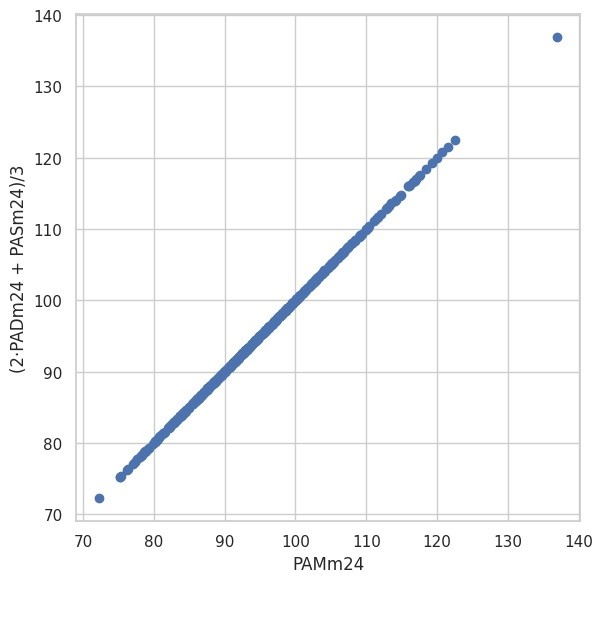
\includegraphics[height=6cm]{./Figures/PAM.jpg}}
	\hspace{1em}
	\subcaptionbox{Relación lineal de PP con PAS y PAD.\label{fig:pp}}
	[0.45\linewidth]{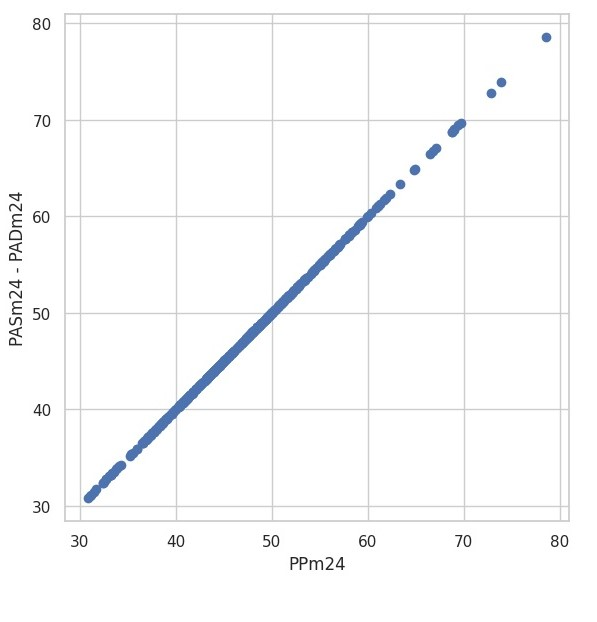
\includegraphics[height=6cm]{./Figures/PP.jpg}}
	\caption{Combinaciones lineales de la presión arterial media y presión de pulso con las presiones sistólicas y diastólicas.}\label{fig:pamypp}
\end{figure}


Teniendo en consideración esta información, se tomó la decisión de no incluir estas variables en 
la red neuronal por diversos motivos. En primer lugar, se buscó evitar la redundancia de información. 
Si una variable es una combinación lineal de otras, significa que la información contenida en 
dicha variable ya está presente en las demás. Por lo tanto, su inclusión solo duplicaría la 
información en la red neuronal, lo cual genera una sobrecarga y ralentiza el proceso de 
entrenamiento. Además, es posible que se generen problemas de inestabilidad numérica puesto que incluso 
pequeñas variaciones en los valores de entrada pueden dar lugar a variaciones significativas 
en las salidas. Esto podría comprometer la estabilidad y precisión de la red neuronal, afectando 
negativamente su rendimiento y capacidad de generar resultados confiables. Otro motivo para 
excluir estas variables es evitar que el modelo se ajuste en exceso a los datos de entrenamiento. 
Es posible que esto resulte en una pérdida de generalización, lo que significa que la red tendría 
dificultades para adaptarse a nuevos datos no vistos anteriormente.

En consecuencia, para abordar estos problemas, se decidió eliminar los valores medios y desviaciones 
estándar de PAM y PP. Así, se preservaron únicamente los valores medidos por el presurómetro: la PAS y PAD. 
De este modo, se asegura que la red neuronal se enfoque en las variables fundamentales y se evitan 
los problemas mencionados anteriormente.

Por otro lado, las variables que incluyen fechas son útiles para brindar fiabilidad a 
la base de datos, ya que proporcionan información sobre el momento en el que se realizó el MAPA y, en caso 
de que hubiese ocurrido, el momento en el que se produjo un evento.
Sin embargo, en el contexto de predecir MACE, estas variables pueden considerarse irrelevantes ya 
que no aportan información sustancial para predecir el resultado deseado. En otras palabras, 
la fecha en sí misma no contiene información directa sobre los atributos fisiológicos o clínicos 
que están más relacionados con la ocurrencia de MACE. Además de su falta de 
relevancia, mantener la variable de fecha agregaría una complejidad adicional al modelo 
de red neuronal. La representación y codificación de la fecha como una característica en el 
modelo requiere un procesamiento adicional. Su transformación en valores numéricos o la 
creación de variables categóricas adicionales aumentaría la dimensionalidad de los datos 
y podría dificultar la interpretación de la red neuronal. Por lo tanto, se decidió eliminar 
esta variable con el fin de agilizar el análisis y entrenamiento de la red neuronal. 

Después de realizar el preprocesamiento a la información proveniente del MAPA, el conjunto 
de datos final utilizado para el desarrollo del modelo incluye las siguientes variables de entrada:

\begin{itemize}
	\item PASm24	
  \item PADm24
  \item FCm24
  \item PASsd24 
  \item PADsd24
  \item FCsd24
  \item PASmDIA
  \item PADmDIA
  \item FCmDIA
  \item htaloadsbpDIA 
  \item htaloaddbpDIA   
  \item HTAdia01	
  \item PASmNOCHE
  \item PADmNOCHE
  \item FCmNOCHE
  \item htaloadsbpNOCHE
  \item htaloaddbpNOCHE
  \item HTAnoche01
\end{itemize}


%%%%%%%%%%%%%%%%%%%%%%%%%%%%%%%%%%%%%%%%%%%%%%%%%%%%%%%%%%%%%%%%%%%%%%%%%%%%%%%%%%%%%%%%%%%%
%%%%%%%%%%%%%%%%%%%%%%%%%%%%%%%%%%%%%%%%%%%%%%%%%%%%%%%%%%%%%%%%%%%%%%%%%%%%%%%%%%%%%%%%%%%%
%------------------------------------------------------------------------
%	datos presurometrias + datos clinicos
\subsection{Conjunto de datos de presurometrías y datos clínicos}
\label{sec:Conjunto2}

El segundo conjunto de datos utilizado incorpora los datos clínicos adicionales de los 491 pacientes que 
se realizaron el MAPA, complementando así la información del conjunto de datos anterior. Dado que muchas 
de las variables son las mismas, esta subsección se enfoca exclusivamente en el preprocesamiento aplicado 
a las nuevas variables clínicas. Estas incluyen 4 variables numéricas (talla, peso, IMC y edad) y 5 variables 
categóricas (sexo, diabetes, tabaquismo, dislipemia e hipertrofia ventricular izquierda).


%%%%%%%%%%%%%%%%%%%%%%%
%%%%%%%%%%%%%%%%%%%%%%%
\subsubsection{Distribuciones de las variables numéricas}
Para analizar las variables clínicas numéricas del conjunto de datos, se llevaron a cabo pruebas visuales y 
estadísticas. En la figura \ref{fig:qqplots2} se exhiben los gráficos Q-Q e histogramas para las variables 
de interés. En cuanto a la talla, se observó que los datos siguen una distribución aproximadamente normal. 
Tanto el gráfico Q-Q como el histograma mostraron una forma de campana característica de esta distribución. 
En el caso del peso y el IMC, se encontró una distribución asimétrica positiva. Esto indica que hay una mayor 
concentración de valores más bajos y una dispersión hacia valores más altos. Esto se debe a que la media y la 
mediana del peso fueron de 76 kg, mientras que la moda se situó en 85 kg. Dado que el IMC se calcula a partir 
del peso y la talla, su distribución sigue una tendencia similar a la del peso. Por otro lado, en cuanto a 
la variable de edad, se identificó una distribución asimétrica negativa. Esto sugiere que existe una mayor 
cantidad de personas mayores en el conjunto de datos. La media de la edad fue de 65 años, con una edad mínima 
de 19 años y una máxima de 98 años. La moda de la distribución se encontró en 72 años.

\begin{figure}[h!]
	\centering
	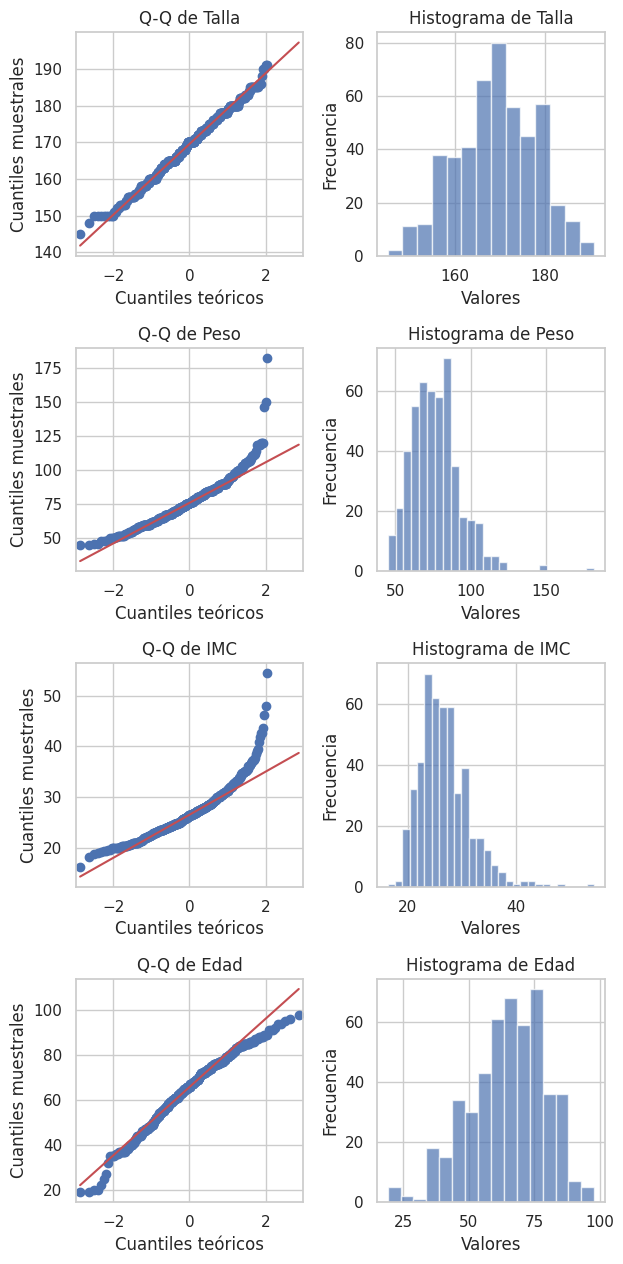
\includegraphics[width=0.7\textwidth]{./Figures/qqplots2.png}
	\caption{Gráficos Q-Q e histogramas de la talla, peso, IMC y edad.}\label{fig:qqplots2}
\end{figure}

Además de los análisis visuales, se realizaron pruebas estadísticas, incluyendo los tests de Shapiro-Wilk 
y Kolmogorov-Smirnov. Los resultados de ambas pruebas indicaron que la talla, el peso y el IMC siguen una 
distribución normal, mientras que la edad no presenta una distribución normal.

%%%%%%%%%%%%%%%%%%%%%%%
%%%%%%%%%%%%%%%%%%%%%%%
\pagebreak 
\subsubsection{Imputación de valores faltantes}
En el segundo conjunto de datos utilizado, se identificaron diferentes variables con valores faltantes. 
A continuación, se detalla la cantidad de valores ausentes en cada una de estas variables:

\begin{itemize}
  \item Sexo: 1 paciente sin información.
  \item Talla, peso e IMC: 9 pacientes sin datos de talla ni peso, lo cual implica la ausencia del cálculo del IMC.
  \item Dislipemia: 1 paciente sin información.
  \item HVI (hipertrofia ventricular izquierda): 2 pacientes sin información.
\end{itemize}

Ante la presencia de estos valores faltantes, es necesario aplicar técnicas de imputación para completar 
la información y garantizar la integridad de los datos. En este trabajo, se optó por utilizar el método 
\emph{KNNImputer} de \emph{scikit-learn} \citep{CITE:50}. Esta elección se basa en la capacidad del método
para capturar la estructura de los datos y aprovechar la información de las instancias vecinas para la 
imputación. Además, este método es adecuado para manejar variables numéricas y categóricas, lo cual es 
relevante en el contexto de este trabajo.

La imputación de datos faltantes utilizando técnicas como el \emph{KNNImputer} desempeña un papel fundamental 
al minimizar la pérdida de información en conjuntos de datos relativamente pequeños, 
como es el caso de este trabajo. De esta manera, se maximiza la utilidad de los datos disponibles y se evita la exclusión 
de observaciones valiosas debido a la falta de información.

%%%%%%%%%%%%%%%%%%%%%%%
%%%%%%%%%%%%%%%%%%%%%%%

\subsubsection{Tratamiento de clases desbalanceadas}

En relación al tratamiento de desbalance de clases, se aplicó el mismo enfoque que en la subsección 
\ref{sec:Conjunto1} debido a que la variable de salida es la misma. Se utilizó la técnica de sobremuestreo 
SMOTE para abordar el desequilibrio de clases y mejorar la representación de la clase minoritaria en el conjunto de datos. 

%%%%%%%%%%%%%%%%%%%%%%%
%%%%%%%%%%%%%%%%%%%%%%%
\subsubsection{Normalización de características}

Para asegurar que todas las características tengan una escala uniforme, se llevó a cabo un proceso de normalización 
de los datos. Al igual que en la subsección \ref{sec:Conjunto1}, se utilizó el método \emph{StandardScaler} \citep{CITE:50}. La 
figura \ref{fig:normalizacion2} presenta las distribuciones antes y después de la normalización de las variables talla, peso, IMC y edad. Este procedimiento garantiza que todas las variables estén en una escala comparable, 
lo que facilita la interpretación y el análisis de los datos para la red neuronal.

\begin{figure}[h!]
	\centering
	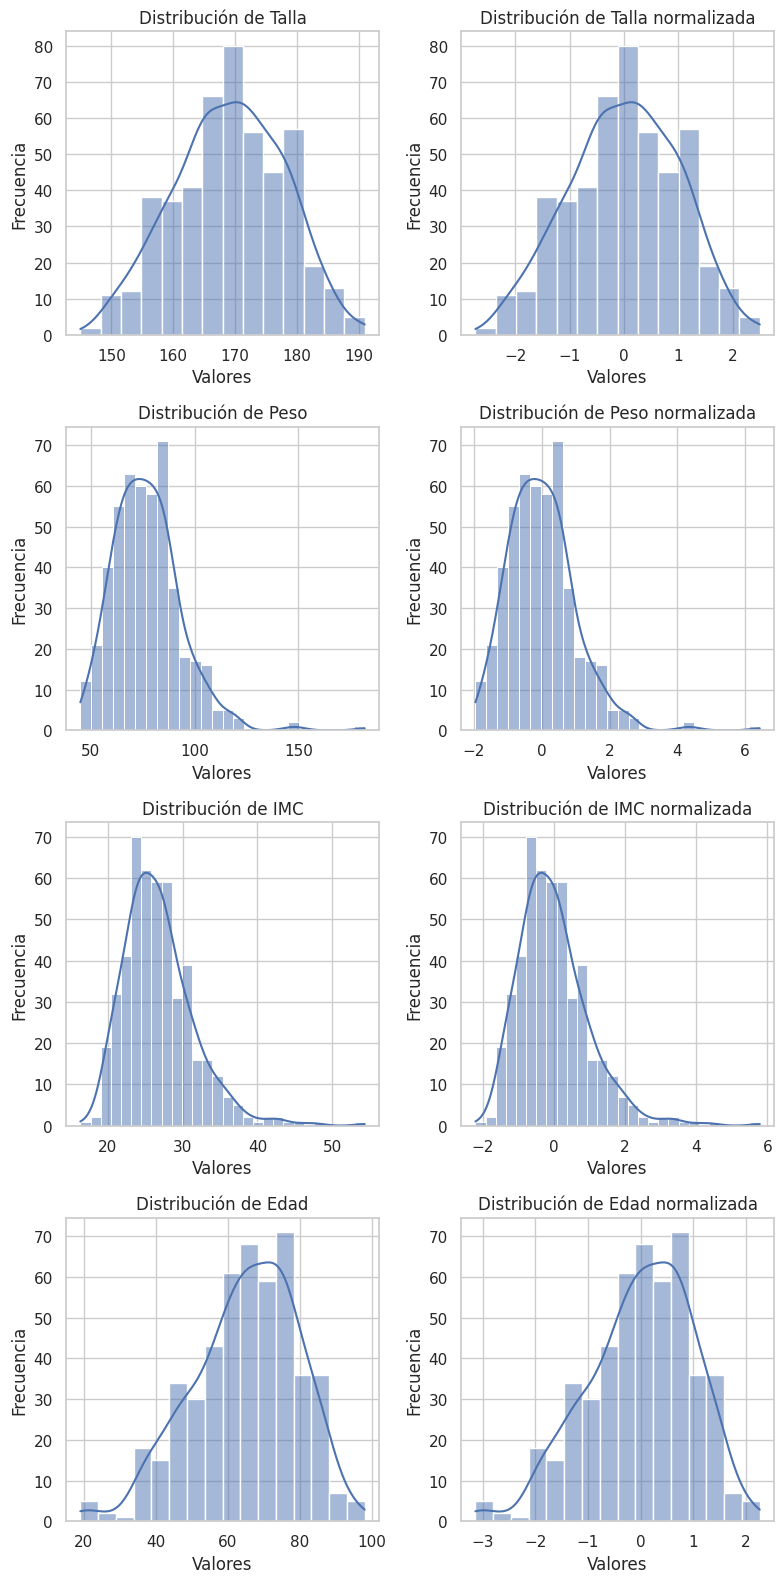
\includegraphics[width=0.7\textwidth]{./Figures/normalizacion2.png}
	\caption{Distribuciones de la talla, peso, IMC y edad antes y después de la normalización.}\label{fig:normalizacion2}
\end{figure}


\filbreak
Después de realizar el preprocesamiento a la información proveniente del MAPA y los datos clínicos, el segundo conjunto de 
datos utilizado para el desarrollo del modelo incluye las siguientes variables de entrada:

\begin{itemize}
  \item PASm24	
  \item PADm24
  \item FCm24
  \item PASsd24 
  \item PADsd24
  \item FCsd24
  \item PASmDIA
  \item PADmDIA
  \item FCmDIA
  \item htaloadsbpDIA 
  \item htaloaddbpDIA   
  \item HTAdia01	
  \item PASmNOCHE
  \item PADmNOCHE
  \item FCmNOCHE
  \item htaloadsbpNOCHE
  \item htaloaddbpNOCHE
  \item HTAnoche01
  \item Talla
  \item Peso
  \item IMC
  \item Edad
  \item Sexo
  \item DBT
  \item Tabaquismo
  \item Dislipemia
  \item HVI
\end{itemize}
